%% For double-blind review submission, w/o CCS and ACM Reference (max submission space)
\documentclass[sigplan,10pt,review]{acmart}
\settopmatter{printfolios=true,printccs=false,printacmref=false}
%% For double-blind review submission, w/ CCS and ACM Reference
%\documentclass[sigplan,review,anonymous]{acmart}\settopmatter{printfolios=true}
%% For single-blind review submission, w/o CCS and ACM Reference (max submission space)
%\documentclass[sigplan,review]{acmart}\settopmatter{printfolios=true,printccs=false,printacmref=false}
%% For single-blind review submission, w/ CCS and ACM Reference
%\documentclass[sigplan,review]{acmart}\settopmatter{printfolios=true}
%% For final camera-ready submission, w/ required CCS and ACM Reference
%\documentclass[sigplan]{acmart}\settopmatter{}


%% Conference information
%% Supplied to authors by publisher for camera-ready submission;
%% use defaults for review submission.
\acmConference[CMPUT 416 Project Final Document]{}{December 2020}{Edmonton, AB, Canada}
\acmYear{2020}
\acmISBN{} % \acmISBN{978-x-xxxx-xxxx-x/YY/MM}
\acmDOI{} % \acmDOI{10.1145/nnnnnnn.nnnnnnn}
\startPage{1}

%% Copyright information
%% Supplied to authors (based on authors' rights management selection;
%% see authors.acm.org) by publisher for camera-ready submission;
%% use 'none' for review submission.
\setcopyright{none}
%\setcopyright{acmcopyright}
%\setcopyright{acmlicensed}
%\setcopyright{rightsretained}
%\copyrightyear{2018}           %% If different from \acmYear

%% Bibliography style
\bibliographystyle{ACM-Reference-Format}
%% Citation style
%\citestyle{acmauthoryear}  %% For author/year citations
%\citestyle{acmnumeric}     %% For numeric citations
%\setcitestyle{nosort}      %% With 'acmnumeric', to disable automatic
                            %% sorting of references within a single citation;
                            %% e.g., \cite{Smith99,Carpenter05,Baker12}
                            %% rendered as [14,5,2] rather than [2,5,14].
%\setcitesyle{nocompress}   %% With 'acmnumeric', to disable automatic
                            %% compression of sequential references within a
                            %% single citation;
                            %% e.g., \cite{Baker12,Baker14,Baker16}
                            %% rendered as [2,3,4] rather than [2-4].


%%%%%%%%%%%%%%%%%%%%%%%%%%%%%%%%%%%%%%%%%%%%%%%%%%%%%%%%%%%%%%%%%%%%%%
%% Note: Authors migrating a paper from traditional SIGPLAN
%% proceedings format to PACMPL format must update the
%% '\documentclass' and topmatter commands above; see
%% 'acmart-pacmpl-template.tex'.
%%%%%%%%%%%%%%%%%%%%%%%%%%%%%%%%%%%%%%%%%%%%%%%%%%%%%%%%%%%%%%%%%%%%%%


%% Some recommended packages.
\usepackage{booktabs}   %% For formal tables:
                        %% http://ctan.org/pkg/booktabs
\usepackage{subcaption} %% For complex figures with subfigures/subcaptions
                        %% http://ctan.org/pkg/subcaption


\begin{document}

%% Title information
\title{Visualizing CodeQL Queries in Visual Studio Code}         %% [Short Title] is optional;
                                        %% when present, will be used in
                                        %% header instead of Full Title.
%\titlenote{with title note}             %% \titlenote is optional;
                                        %% can be repeated if necessary;
                                        %% contents suppressed with 'anonymous'
%\subtitle{Subtitle}                     %% \subtitle is optional
%\subtitlenote{with subtitle note}       %% \subtitlenote is optional;
                                        %% can be repeated if necessary;
                                        %% contents suppressed with 'anonymous'


%% Author information
%% Contents and number of authors suppressed with 'anonymous'.
%% Each author should be introduced by \author, followed by
%% \authornote (optional), \orcid (optional), \affiliation, and
%% \email.
%% An author may have multiple affiliations and/or emails; repeat the
%% appropriate command.
%% Many elements are not rendered, but should be provided for metadata
%% extraction tools.

%% Author with single affiliation.
\author{Jacob Skitsko}
%\authornote{with author1 note}          %% \authornote is optional;
                                        %% can be repeated if necessary
\orcid{nnnn-nnnn-nnnn-nnnn}             %% \orcid is optional
\affiliation{
  %\position{Position1}
  %\department{Department1}              %% \department is recommended
  \institution{University of Alberta}            %% \institution is required
  %\streetaddress{Street1 Address1}
  %\city{City1}
  %\state{State1}
  %\postcode{Post-Code1}
  %\country{Country1}                    %% \country is recommended
}
\email{jskitsko@ualberta.ca}          %% \email is recommended

%% Author with two affiliations and emails.
\author{Robert MacGillivray}
%\authornote{with author2 note}          %% \authornote is optional;
                                        %% can be repeated if necessary
%\orcid{nnnn-nnnn-nnnn-nnnn}             %% \orcid is optional
\affiliation{
  %\position{Position2a}
  %\department{Department2a}             %% \department is recommended
  \institution{University of Alberta}           %% \institution is required
  %\streetaddress{Street2a Address2a}
  %\city{City2a}
  %\state{State2a}
  %\postcode{Post-Code2a}
  %\country{Country2a}                   %% \country is recommended
}
\email{rmacgill@ualberta.ca}         %% \email is recommended

%% Author with two affiliations and emails.
\author{Cijie Xia}
%\authornote{with author2 note}          %% \authornote is optional;
                                        %% can be repeated if necessary
%\orcid{nnnn-nnnn-nnnn-nnnn}             %% \orcid is optional
\affiliation{
  %\position{Position2a}
  %\department{Department2a}             %% \department is recommended
  \institution{University of Alberta}           %% \institution is required
  %\streetaddress{Street2a Address2a}
  %\city{City2a}
  %\state{State2a}
  %\postcode{Post-Code2a}
  %\country{Country2a}                   %% \country is recommended
}
\email{cijie@ualberta.ca}         %% \email is recommended



%% Abstract
%% Note: \begin{abstract}...\end{abstract} environment must come
%% before \maketitle command
\begin{abstract}
CodeQL is a program analysis tool developed by Github Security Lab. Developers and researchers can identify software vulnerabilities and bugs with CodeQL by writing powerful queries  called QL. GitHub also developed a CodeQL Visual Studio Code extension, which is an open source project written in TypeScript, utilizing the CodeQL command line tool for the analysis service. This extension currently displays the analysis results in the tabular view. 
\newline
\indent In this paper, we present CodeQLVis - a CodeQL visualization tool integrated in Visual Studio Code which creates intuitive graphical representations of the analysis results from CodeQL. 

\end{abstract}


%% 2012 ACM Computing Classification System (CSS) concepts
%% Generate at 'http://dl.acm.org/ccs/ccs.cfm'.
\begin{CCSXML}
<ccs2012>
<concept>
<concept_id>10011007.10011006.10011008</concept_id>
<concept_desc>Software and its engineering~General programming languages</concept_desc>
<concept_significance>500</concept_significance>
</concept>
<concept>
<concept_id>10003456.10003457.10003521.10003525</concept_id>
<concept_desc>Social and professional topics~History of programming languages</concept_desc>
<concept_significance>300</concept_significance>
</concept>
</ccs2012>
\end{CCSXML}

\ccsdesc[500]{Software and its engineering~General programming languages}
\ccsdesc[300]{Social and professional topics~History of programming languages}
%% End of generated code


%% Keywords
%% comma separated list
\keywords{Program Analysis, Developer Tools, Visualization}  %% \keywords are mandatory in final camera-ready submission


%% \maketitle
%% Note: \maketitle command must come after title commands, author
%% commands, abstract environment, Computing Classification System
%% environment and commands, and keywords command.
\maketitle


\section{Introduction and Motivation}
CodeQL is a powerful code analysis engine that supports many mainstream programming languages such as Java, C\#, Python, JavaScript and more. Developers are able to use CodeQL to quickly perform data-flow analyses on their programs and identity software vulnerabilities such as taint flows, or to acquire programs' properties such as call graphs. 
\newline
\indent Existing tools leveraging CodeQL on the market display the analysis results only in text-based methods, which is not very straightforward and requires users to have knowledge in program analysis to understand. For example, LGTM has tools that make it easier to understand data-flow analysis performed with CodeQL. The way they explore data flow paths is with a series of code snippets. CodeQL Visual Studio Code extension only outputs the analysis results in tabular view.
\newline
\indent Semmle, the company behind CodeQL, has been acquired by GitHub and widespread public support for CodeQL has resulted. The popularity of this tool, and the lack of visualization support, has given us reason to explore this problem. We've narrowed our scope in this domain to visualizing dataflow analysis, particularly as it pertains to taint-flow tracking. 
\newline
\indent Therefore, in order to convey a complete and intuitive picture of a system more quickly than text-based methods, we have extended the CodeQL for Visual Studio Code extension to support taint-flow graph visualizations.

\begin{figure}[h]
  \centering
  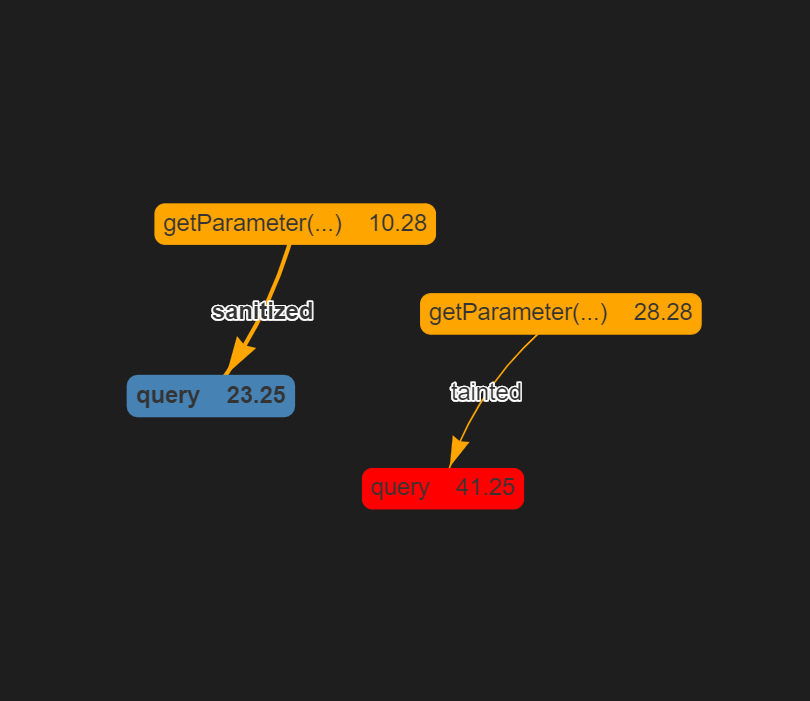
\includegraphics[width=\linewidth]{taint_part}
  \caption{Taint Analysis Visualization. Only the necessary part of the taint flow path is shown. Orange denotes the source. Yellow denotes the data that is tainted. Red denotes the sink. Dark blue denotes the sink that is sanitized. Light blue denotes the data that is not tainted.}
\end{figure}

\begin{figure}[h]
  \centering
  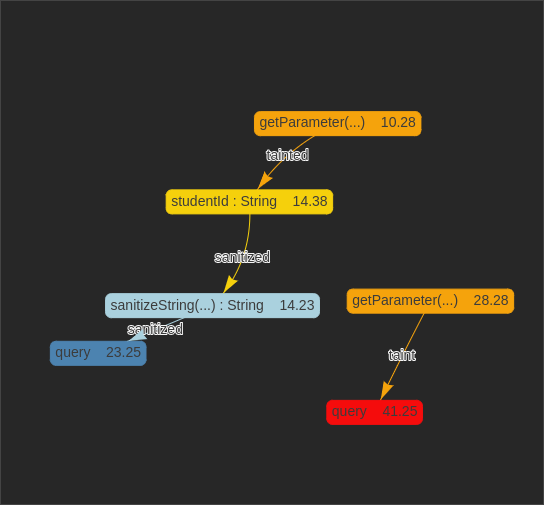
\includegraphics[width=\linewidth]{taint_full}
  \caption{Full path of the taint flow. }
\end{figure}

\section{Background}
\textcolor{red}{We'll probably want to extend this section with any bits of terminology that we use later on. If we need to add a third section for another foundational element, we can do that as well.\newline}
Our work is heavily dependent upon the static analysis tool CodeQL, as well as the framework for Visual Studio Code extensions. As such, we will provide a brief introduction to both of these to better contextualize our artifact.
\subsection{CodeQL}
CodeQL is a tool for performing static analysis that transforms code into queryable relational databases. Database queries are then written in the CodeQL language to retrieve certain properties about the code that the database was derived from. This approach makes CodeQL incredibly fast, though the free-form nature of database queries means that it can be difficult to know exactly what format the data will have when retrieved.
\newline
\indent Two queries with the same semantic meaning can retrieve sets of data that are superficially different. As a result, there are efforts underway to produce libraries of pre-defined queries to help users look for common vulnerabilities or other issues in their code-base.
\subsection{Visual Studio Code Extensions}
Visual Studio Code extensions are in-editor tools that are created by their community of users. Visual Studio Code, often abbreviated to VS Code, offers a powerful Extension API for this purpose. Extensions are written in JavaScript or TypeScript and can modify almost any aspect of VS Code. Features such us simple editor themes, all the way to adding support for self-developed programming languages is possible.
\newline
\indent Of particular interest for our purposes are VS Code Webviews. Where an extension that has been limited to the Extensions API are limited to modifying existing elements of the editor, the Webview API provides an opportunity to render interactive HTML in order to create entirely new functionality within the editor. CodeQL for Visual Studio Code, for example, uses this API to render query results tables.

\section{Overview}
Thanks to the fact that CodeQL VSCode extension is open sourced, we built our visualization tool by extending this existing CodeQL extension. For the visualization part, we utilized the WebView APIs provided by VSCode and visualization libraries available for rendering the UI. 
\newline
\indent CodeQLVis will be provided as an alternative to CodeQL VSCode extension's default way of redering the results in tabular view. Users can easily switch between using the default or CodeQLVis. More details of the implementation of CodeQLVis will be described in the following section.

\begin{figure}[h]
  \centering
  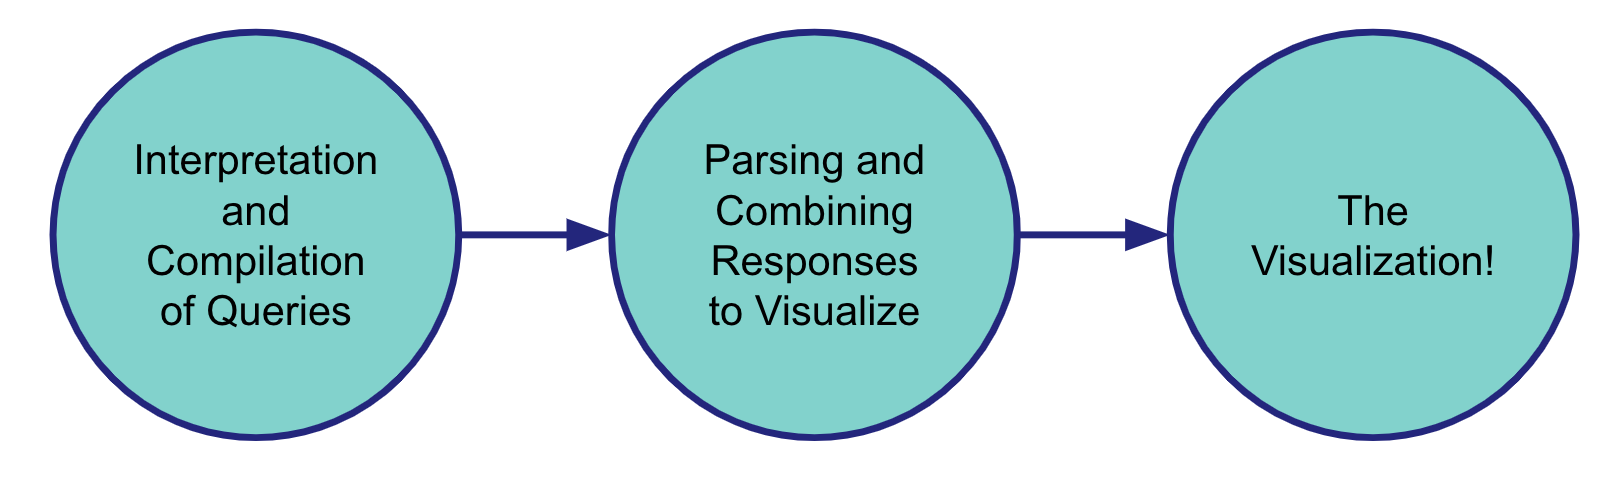
\includegraphics[width=\linewidth]{work_flow}
  \caption{The work flow}
\end{figure}

\section{Approach}
\subsection{CodeQL Queries}
\[TODO\] 
\subsection{Queries to Graphs}
\[TODO\] 
\subsection{Rendering Results}
\[TODO\] 

\section{Evaluation}
\[TODO\] 

\section{Discussion}
\[TODO\]

\section{Related Work}
\textcolor{red}{Probably get rid of the related tools bit. Everything we could say here fits better in the background. Expand Data Flow Visualization section such that each entry gets it's own bolded section.\newline}
There are a few tools which we have leveraged in order to make our work possible. In addition, there have been some taint flow visualization efforts using other static analysis tools that we would like to highlight.
\newline
\newline
\indent \textbf{Related Tools}. CodeQL is integral to our efforts as the program analysis tool which produces results for us to visualize. CodeQL for Visual Studio Code is cool. VS Code Debug Visualizer is also cool.
\newline
\newline
\indent \textbf{Data Flow Visualization}. There are a number of efforts in this domain, though not necessarily applied to CodeQL nor integrated into Visual Studio Code. "Understanding and Visualizing Full Systems with
Data Flow Tomography" outlines an approach whereby data is tagged and tracked through the program to develop a visualzation of all interconnected pieces. In contrast, rather than doing live analysis, we use CodeQL to perform static analysis and find theoretical data flow paths that meet certain pre-defined criteria. "VisuFlow" is a plugin developed for the Eclipse IDE that generates visualizations for static analysis performed by Soot. While similar to our approach, their plugin does not work with CodeQL queries, and was developed for a different IDE.
\[TODO\] 

\section{Conclusion}
\textcolor{red}{Expand this.\newline}
We have shown a possible route to extend CodeQL for Visual Studio Code, offering a visual representation of data that is otherwise typically presented in tabular format. This optional visualization has been further broken down into different levels of granularity per a user's preference for a given query. Our approach leverages the source extension such that we can interpret taint-flow analysis queries of specific formats, subtly modifying queries before execution where necessary.
\newline
\indent
This proof of concept shows promise; though, as we have discussed, the limitations are numerous and obvious at this stage. It is our opinion that it will be possible to refine our approach in order to make CodeQL more accessible and intuitive to use for developers regardless of their potential lack of foundational knowledge in static analysis.
\[TODO\]

\end{document}
